\section{Question 3}

\subsection{Question}
\verbatiminput{q3/q3.txt}

\subsection{Answer}
To give an idea of the overall layout of the graph refer to Figure \ref{fig:overview}. 

\begin{figure}[h!]
\centering
\fbox{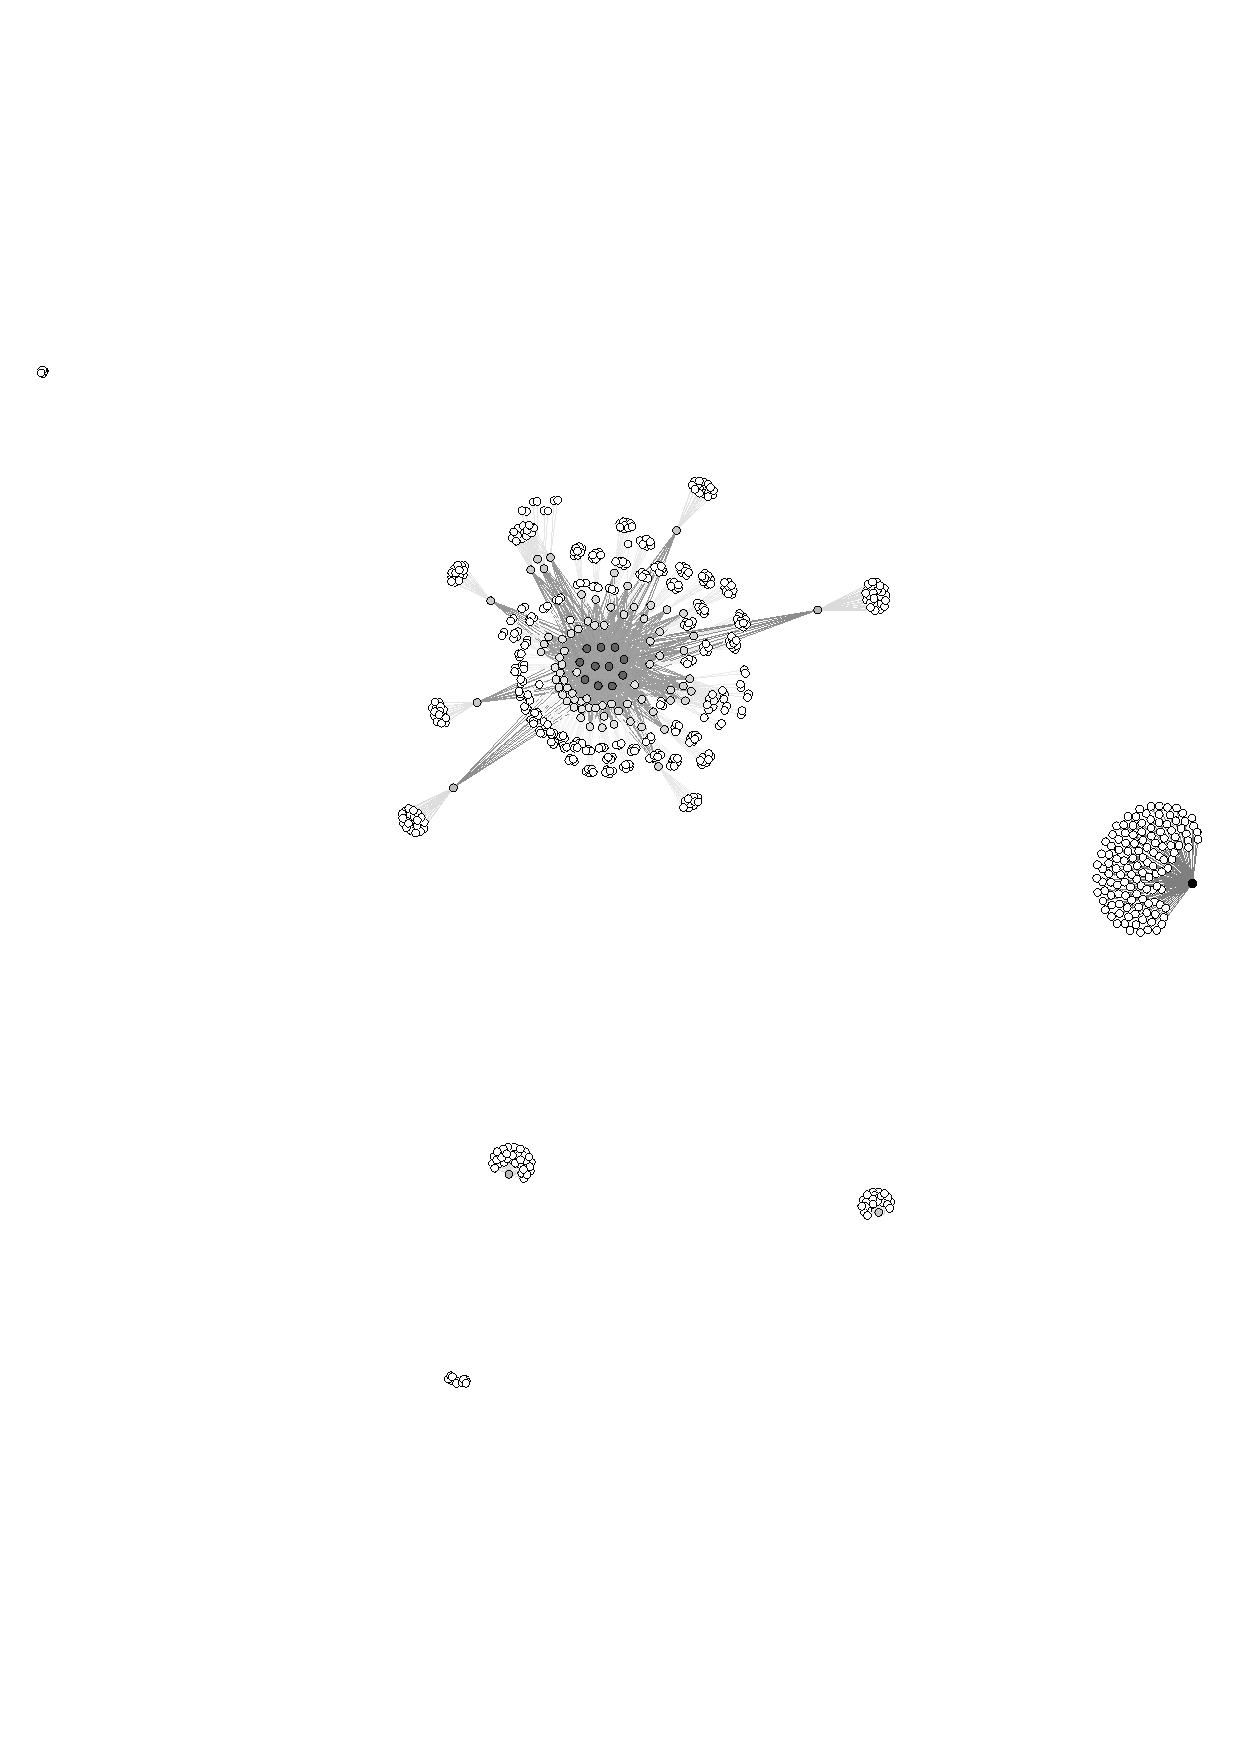
\includegraphics[trim=0 150 0 150, clip, scale=0.35]{q3/graphs/overview.pdf}}
\caption{Graph Overview}
\label{fig:overview}
\end{figure}

\clearpage

The graph has one strongly connected core component with a few chunked islands of links not connected to the core. The strongly connected component is shown closer in Figure \ref{fig:core}.

\begin{figure}[h!]
\centering
\fbox{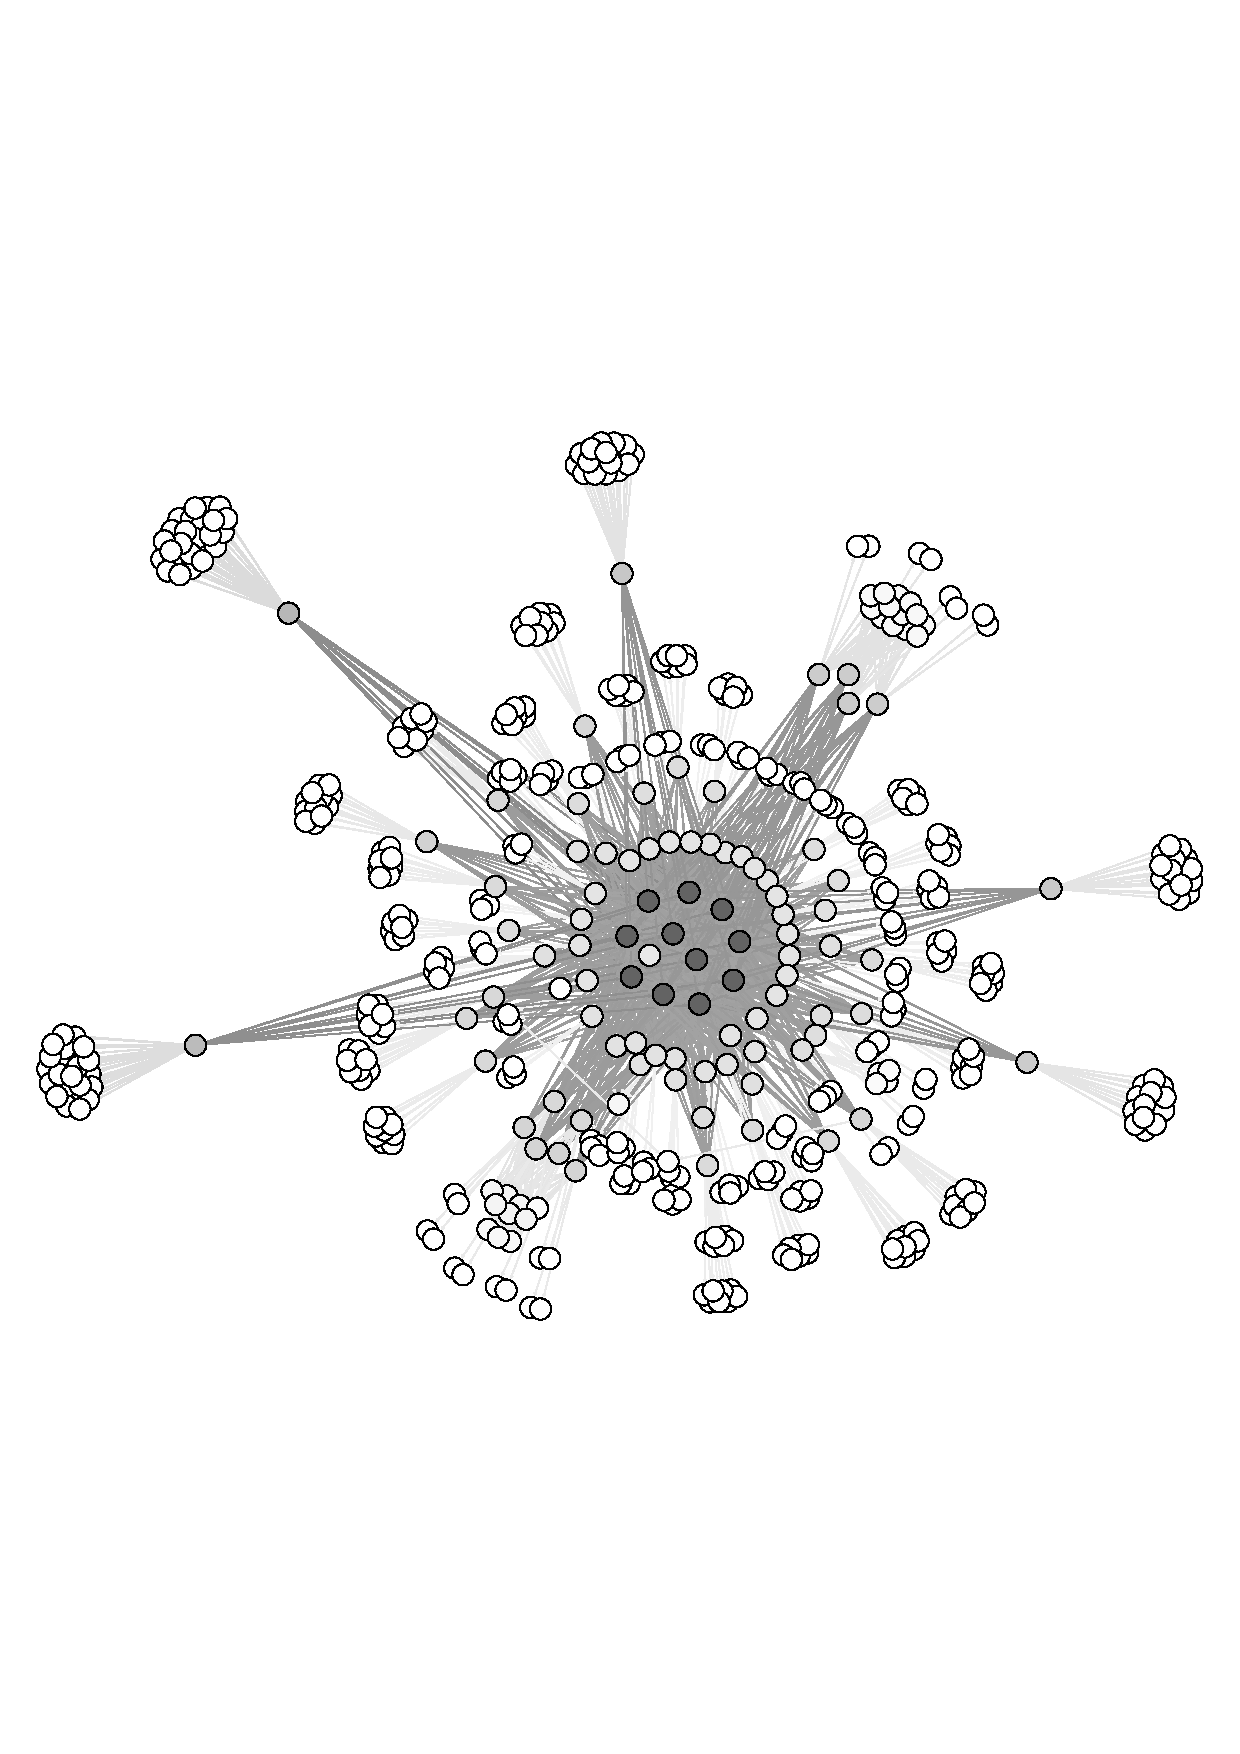
\includegraphics[trim=0 150 0 150, clip, scale=0.5]{q3/graphs/core.pdf}}
\caption{Strongly Connected Core}
\label{fig:core}
\end{figure}

The nodes in the center are mostly from google domains -- YouTube.com, various google.com sub-domains, like plus.google.com, accounts.google.com, etc. This core is illustrated with node labels in Figure \ref{fig:coreclose}. The core is well connected, presumably because they are domains controlled by a single company that is involved in connecting their users with a multitude of online resources. 

\begin{figure}[h!]
\centering
\fbox{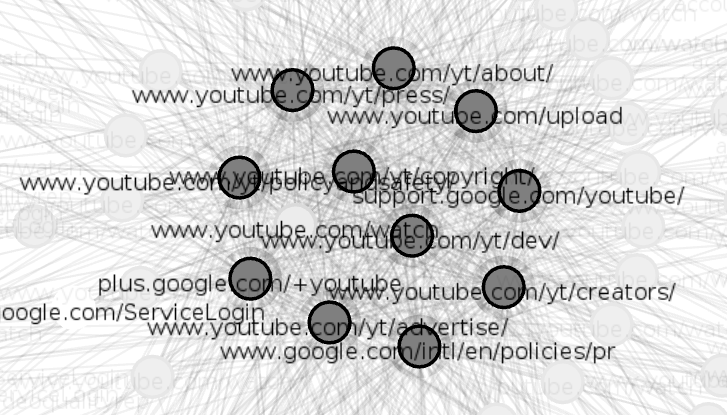
\includegraphics[scale=0.3]{q3/graphs/core_close_labels.png}}
\caption{Core Close-up}
\label{fig:coreclose}
\end{figure}

\clearpage

The Hyperlink-Induced Topic Search (HITS) is a graph analysis algorithm that ranks nodes in a connected graph based on two categories: authorities and hubs. A high authority score means that the page is pointed to by many hubs and a high hub score means the page points to many authorities. The algorithm was run on the sample graph created and the results are displayed in Figures \ref{fig:authorities} and \ref{fig:hubs}.

\begin{figure}[h!]
\centering
\fbox{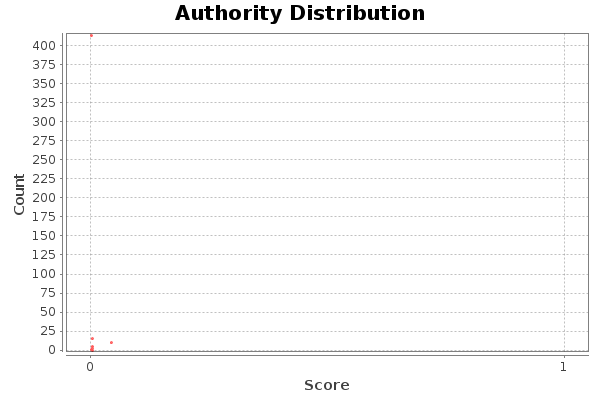
\includegraphics[scale=0.5]{q3/graphs/hits/authorities.png}}
\caption{HITS Authorities Scores}
\label{fig:authorities}
\end{figure}

\begin{figure}[h!]
\centering
\fbox{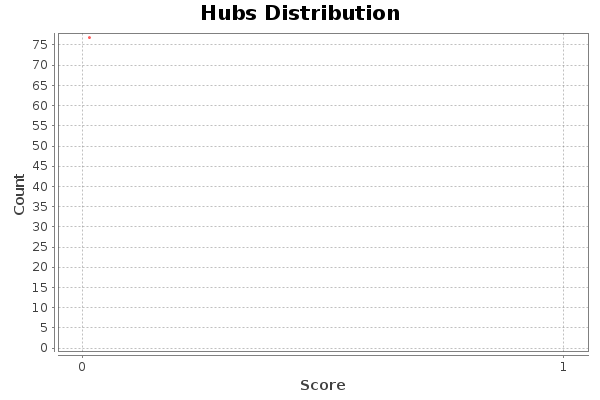
\includegraphics[scale=0.5]{q3/graphs/hits/hubs.png}}
\caption{HITS Hubs Scores}
\label{fig:hubs}
\end{figure}

\clearpage

Page Rank is an algorithm that is used to measure the importance of a node in a connected graph, used to rank web pages in an order search result. It was developed by Google for use in its search engine of the same name. It is basically a valuation measure of each page found by adding up the degree for each page and normalizing it against the rest of the pages in the set. The algorithm was run on the sample graph created and the results are displayed in Figure \ref{fig:pagerank}

\begin{figure}[h!]
\centering
\fbox{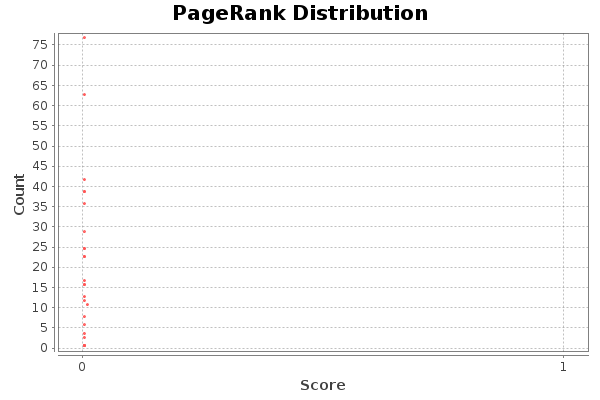
\includegraphics[scale=0.5]{q3/graphs/pagerank/pageranks.png}}
\caption{Page Rank Scores}
\label{fig:pagerank}
\end{figure}

The average degree of the graph was also calculated. The results are found in Figures \ref{fig:degree}, \ref{fig:indegree} and \ref{fig:outdegree}.

\begin{figure}[h!]
\centering
\fbox{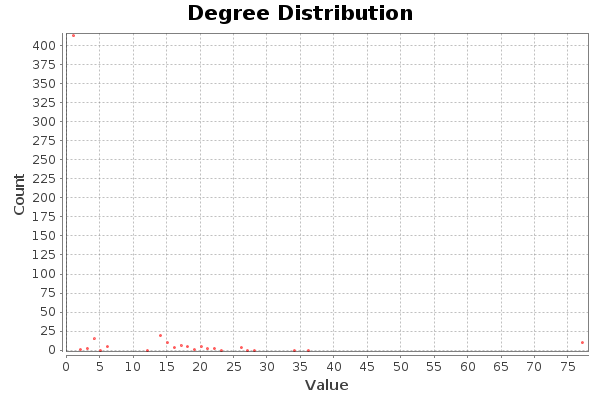
\includegraphics[scale=0.5]{q3/graphs/degree/degree-distribution.png}}
\caption{Average Degree Distributions}
\label{fig:degree}
\end{figure}

\begin{figure}[h!]
\centering
\fbox{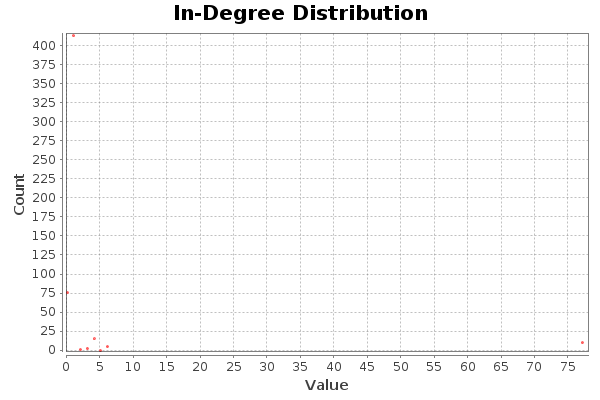
\includegraphics[scale=0.5]{q3/graphs/degree/indegree-distribution.png}}
\caption{In-Degree Distributions}
\label{fig:indegree}
\end{figure}

\begin{figure}[h!]
\centering
\fbox{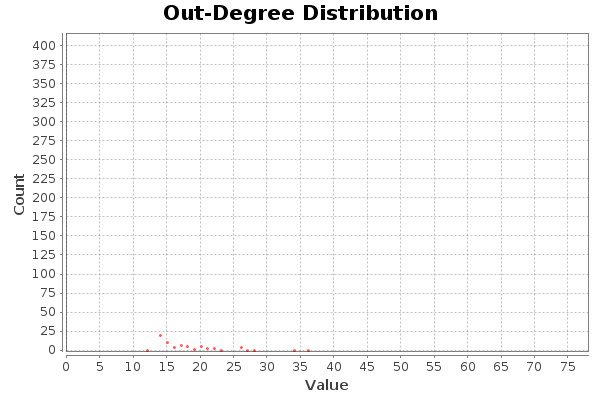
\includegraphics[scale=0.5]{q3/graphs/degree/outdegree-distribution.png}}
\caption{Out-Degree Distributions}
\label{fig:outdegree}
\end{figure}

\clearpage

The network diameter was calculated and the results are found in Figures \ref{fig:between}, \ref{fig:closeness} and \ref{fig:eccentricity}.

\begin{figure}[h!]
\centering
\fbox{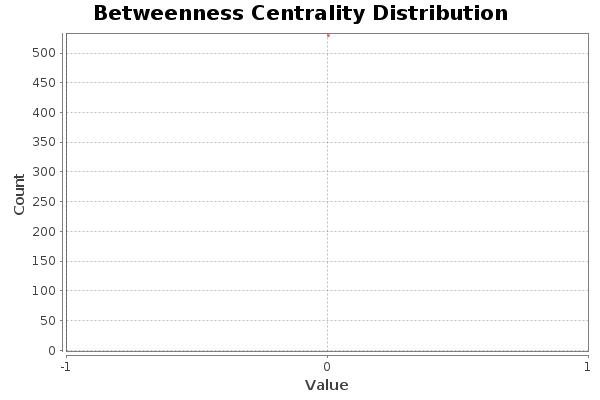
\includegraphics[scale=0.5]{q3/graphs/diameter/betweenness_centrality_distribution.png}}
\caption{Betweenness Centrality Distribution}
\label{fig:between}
\end{figure}

\begin{figure}[h!]
\centering
\fbox{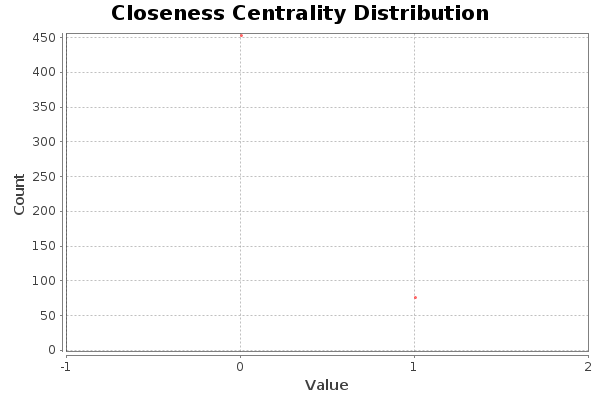
\includegraphics[scale=0.5]{q3/graphs/diameter/closeness_centrality_distribution.png}}
\caption{Closeness Centrality Distribution}
\label{fig:closeness}
\end{figure}

\clearpage

\begin{figure}[h!]
\centering
\fbox{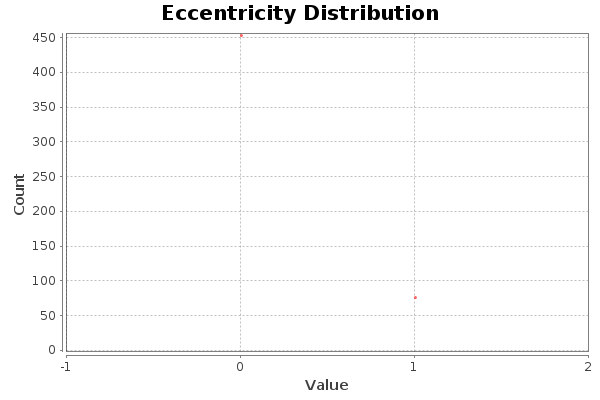
\includegraphics[scale=0.5]{q3/graphs/diameter/eccentricity_distribution.png}}
\caption{Eccentricity Distribution}
\label{fig:eccentricity}
\end{figure}

The connected components were found. The results are in Figure \ref{fig:connected}

\begin{figure}[h!]
\centering
\fbox{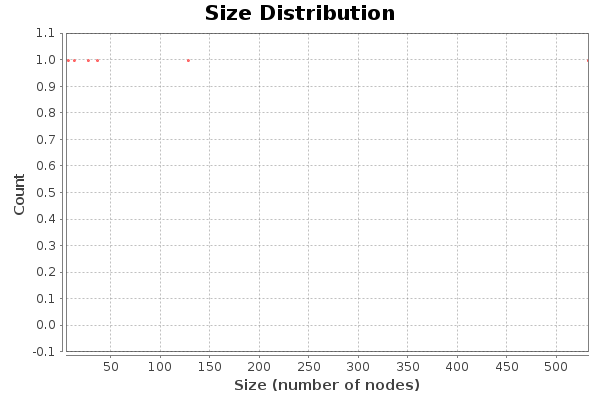
\includegraphics[scale=0.5]{q3/graphs/connected_components/cc-size-distribution.png}}
\caption{Connected Components}
\label{fig:connected}
\end{figure}